\documentclass[dvipsnames] {beamer}
\usepackage{cmlgc}
\usepackage{comment}
\usepackage{tikz}
\usefonttheme{serif}     % Font theme: serif
\usepackage[T2A]{fontenc}
\usepackage[utf8]{inputenc}
\usepackage[english,russian]{babel}
\usepackage{amssymb,amsfonts,amsmath,mathtext,cite,enumerate,float} %подключаем нужные пакеты расширений
% \usepackage{cyrillic}
\usepackage{color, colortbl}
\usepackage{multirow}
\usepackage{graphicx}
\usepackage{graphics}
\usepackage{multirow}
\usepackage{url}
\usepackage{hyperref}
\usepackage{animate}
\usepackage{pifont}
\usepackage{wasysym}
\usepackage{marvosym}
\usepackage{appendixnumberbeamer} 
\usepackage{pgfpages}


\usepackage{ragged2e} %выравнивание текста по ширине слайда (\justifying)
%\setbeamercolor{background canvas}{bg=violet}

\usetheme{AnnArbor}
\usecolortheme{crane}

%=================================================

    \defbeamertemplate*{footline}{mytheme}{%
      \leavevmode%
      \hbox{%
      \begin{beamercolorbox}[wd=.2\paperwidth,ht=3ex,dp=1ex,center]{author in head/foot}%
        \usebeamerfont{author in head/foot}\insertshortauthor
      \end{beamercolorbox}%
      \begin{beamercolorbox}[wd=.7\paperwidth,ht=3ex,dp=1ex,center]{title in head/foot}%
        \usebeamerfont{title in head/foot}\insertshorttitle
      \end{beamercolorbox}%
      \begin{beamercolorbox}[wd=.1\paperwidth,ht=3ex,dp=1ex,right]{date in head/foot}%
        %\usebeamerfont{date in head/foot}\insertshortdate{}\hspace*{2em}
        %\insertframenumber{} / \inserttotalframenumber\hspace*{2ex} %номер текущего слайда / общее число слайдов
        \insertframenumber{} \hspace*{5ex}  %номер текущего слайда
      \end{beamercolorbox}}%
      \vskip0pt%
    }
    \usebeamertemplate{mytheme}


\defbeamertemplate*{frametitle}{boldTitle}{%
    \begin{beamercolorbox}[wd=\paperwidth,ht=3ex,dp=3pt,center]{title in head/foot}%
%        \ \textit{\textbf{\insertframetitle}} % курсивный заголовок слайда 
        \ \textbf{\insertframetitle}
    \end{beamercolorbox}
}
\usebeamertemplate{boldTitle}
\setbeamercovered{dynamic}

%\setbeameroption{hide notes} % Only slides
%\setbeameroption{show only notes} % Only notes
%\setbeameroption{show notes on second screen=right} % Both
%\setbeamertemplate{note page}[plain]


%=================================================
% \titlegraphic{
\includegraphics[width=\textwidth]{logo_conf.png}}
\addtobeamertemplate{title page}{\centering 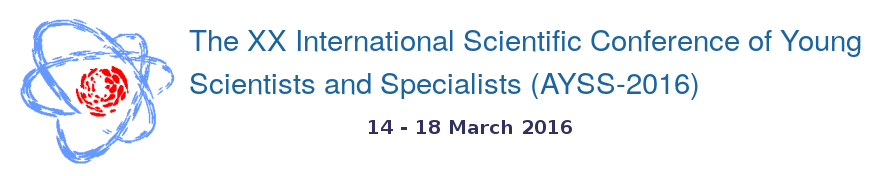
\includegraphics[scale=0.39]{ayss2016_logo.png}}{}
\title[ Femtoscopy, NICA, MPD ...]{\textbf{\large {Feasibility of femtoscopy studies at the NICA energies}}}

%\author[P.~Batyuk]{\textit{\textbf{{\footnotesize \underline{P.~Batyuk}, L.~Malinina (SINP MSU, JINR), \\ O.~Rogachevskiy (JINR)}}} \\
%  on behalf of the MPD collaboration}
\author[P.~Batyuk]{\textit{\textbf{{\footnotesize \underline{P.~Batyuk}, L.~Malinina, D.~Wielanek}}}} 
\institute{\url{pavel.batyuk@jinr.ru}  \\ VBLHEP, JINR}

\date{{\textbf{Section 1: High energy physics} \\ 
 \newpage \footnotesize March 16, 2016}}

\graphicspath{{../common_figures/}}

\begin{document}
\maketitle
\note{On behalf of the MPD collaboration I would like to present you a report on ``Feasibility of femtoscopic analysis for the MPD''.}

\begin{frame}
  \frametitle{Outline}
  \begin{itemize}
    \bf 
  \item Introduction
%  \item Physics Motivation
  \item Femtoscopy at different energies: from STAR to NICA
  \item Source function technique
  \item Conclusion
  \end{itemize}
  \note{
    A short plan of the report is presented in the slide.
    The report will be consisting of two parts.
    In the first part I will observe the well developed formalism of femtoscopic studies.
    Also, a technique called "source imaging'' will be discussed and considered as a
    way to see the detailed structure of source deviating from the Gaussian distribution and having a more
    complicated form.
    \\
    In the second part some preliminary femtoscopic investigations within the MPD are discussed.
    The main impact is concentrated on effects distorting the obtained CFs. 
  }
\end{frame}

\begin{frame}
  \frametitle{Introduction}
  \begin{columns}[c]
    \column{.20\textwidth}
    \begin{block}{}
      \begin{figure}[H]
        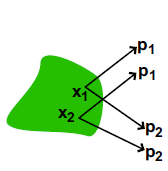
\includegraphics[width=0.8\linewidth]{corr_femto1.png}
      \end{figure}
    \end{block}
    \column{.70\textwidth}
    \begin{block}{{\bf Correlation femtoscopy:}}
      Measurement of space-time characteristics $R$, $c_{\tau}$ (fm) of particle production
      using particle correlations due to the effects of quantum statistics (QS) and final state interactions (FSI)
    \end{block}
  \end{columns}

  \begin{columns}[c]
    \column{.40\textwidth}
    \begin{block}{}
      \begin{figure}[H]
        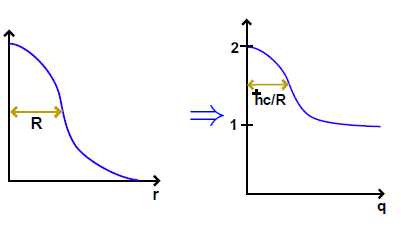
\includegraphics[width=0.8\linewidth]{corr_femto2.png}
      \end{figure}
    \end{block}
    \column{.50\textwidth}
    \begin{block}{{\bf \centering Two-particle correlation function:}}
      \tiny{
        \begin{center}
          {\bf theory:     $C(q) = \dfrac{N_{2}(p_{1}, p_{2})}{N_{1}(p_{1}) N_{2}(p_{2})}, C(\infty) = 1$
        
            experiment: $C(q) = \dfrac{S(q)}{B(q)}, q = p_{1} - p_{2}$
            
            \alert {S(q)} is a distribution of pair momentum difference of particles from the same event
            
            \alert {B(q)} is a reference distribution built by mixing of particles from different events}
        \end{center}
      }
    \end{block}
  \end{columns}
  \note{
    { \footnotesize
    Size and temporal parameters of the particle-emitting region at freeze-out can be
    extracted by use of femtoscopic techniques. 
    Momentum correlations of two particles at small relative momenta
    in their center-of-mass system (CMS) are widely used for studying space-time
    characteristics of heavy-ion collisions on a level of $10^{-15}$ m,
    giving a correlation femtoscopy tool.
    The femtoscopic correlations due to quantum statistics (QS)
    of the produced identical particles were observed more than 50 years
    ago as an enhanced production of pairs of identical
    pions with small opening angles. 
    A general base of the modern correlation femtoscopy was
    proposed by Kopylov and Podgoretsky (JINR, Dubna) in early 70th of the previous century.
    %Moreover, the femtoscopic correlations, along with the space-time
    %characteristics of particle production, give also an information on low-energy strong interaction between specific
    %particles, which can be hardly achieved by other techniques.

    The femtoscopiс correlations of two identical particles can be described by using a two-particle correlation function.
    Experimentally, it is defined as a ratio of two functions depending on pair momentum difference $\bf q$,
    where S(q) is a ..., and B(q) is a ...   
    
    }
  }
\end{frame}



\begin{frame}
  \frametitle{Introduction}
  \begin{block}{}
    \tiny{ \bf
      The main goal of experiments with heavy ion collisions is to study the new forms of matter which can be created under the extreme
      conditions at the early stage of the evolution.
    }
  \end{block}
  \begin{block}{}
    \begin{figure}[H]
      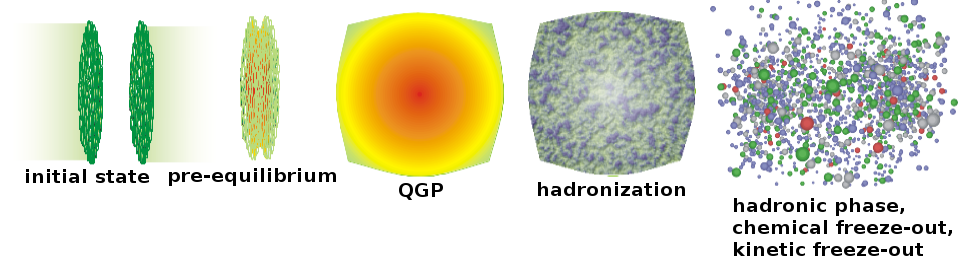
\includegraphics[width=0.8\linewidth]{corr_femto3.png}
    \end{figure}
  \end{block}
  \begin{block}{}
    \tiny{ \bf
    \begin{itemize}
    \item Information on the space-time evolution can only be extracted by study the femtoscopy correlations.
    \item The correlations depend on the space-time distance separating emission points and on the particle relative momentum.
    \item The space-time relative distances are measured at the points where the particles stop to interact, then they are set
      free (kinetic freeze-out). This moment occurs at very late stage of collisions after the QGP was created and disappeared.
    \item The available signals (geometric growth of the reaction zone, the specific features of the collective flow generated by the
      QGP pressure gradients) are revealed in the final state as very specific space-momentum correlations influencing particle spectra
      and correlation radii.
    \end{itemize}
    }
  \end{block}
  \note{
    { \footnotesize
      In case of experiments dealing with HI-collisions one of the main goals is related to a study of the new forms of matter
      forming under extreme temperatures and densities that take place within the early stage of evolution.
      It should be stressed that information on space-time evolution of the colliding system can be extracted by the femtoscopic
      correlations only. These correlations depend on \\
      - the space-time distance separating emission points \\
      - the particle relative momentum \\
      The space-time relative distances are measured at the points where the particles stop to interact. Despite this moment occurs at very
      late stage of collisions after the QGP was created and disappeared, available signals mentioned in the slide could be
      observed as very specific space-momentum correlations that affect particle spectra and correlation radii.
    }
  }
\end{frame}

\begin{frame}
  \frametitle{Femtoscopy: parametrizations used}
  \begin{block}{}
   
      \centering {
        $C(q) = 1 + \lambda e^{-R_{inv}^{2} q_{inv}^{2}}$
        \tiny{ \bf
          
          $\lambda$ is a correlation strength,
          
          $R_{inv}$ assumes a Gaussian radius in the Pair Reference Frame (PRF)
          
          \small {\alert{1d-analysis}} is sensitive only to the system size averaged over all directions.

        }
      }
    
  \end{block}
  \begin{block}{}
  
      \centering {
        $C(q) = 1 + \lambda e^{-R_{out}^{2}q_{out}^{2} - R_{side}^{2}q_{side}^{2} - R_{long}^{2}q_{long}^{2}}$
        \tiny{ \bf

        $R, q$ are defined in the Longitudinally Co-Moving Frame (LCMS)
        
        \small {\alert{3d-analysis}} gives an access to the three system sizes in three directions separately.

        }
      }
  \end{block}

  \begin{columns}[c]
    \column{.4\textwidth}
     \begin{block}{\center \bf Definition of femtoscopic radii:}
       \begin{figure}[H]
      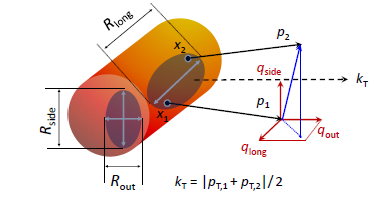
\includegraphics[width=0.7\linewidth]{corr_femto4.png}
       \end{figure}
     \end{block}
     \column{.5\textwidth}
     \begin{block}{\center \bf 3D-analysis:}
       \footnotesize{
       $R_{side}$ is sensitive to {\bf geometrical transverse size}
       \newline
       $R_{long}$ is sensitive to {\bf time of freeze-out}
       
       $R_{out} / R_{side }$ is sensitive to {\bf emission duration}
       }
     \end{block}
  \end{columns}
  \note{
    {\tiny
      The developed femtoscopic techniques allow one for performing two types of the analysis: 1D and 3D.
      In case of the 1D femtoscopic analysis CF is parametrized as presented in the slide. 
      But this analysis has a small disadvantage: it gives the system size averaged over all directions.
      In case of the 3D femtoscopic analysis pair relative momentum $\bf q$ can be expanded into three components shown schematically in the slide.
      It gives an access to the three system sizes in three directions
      separately. $\bf q$ is expanded into the longitudinal component $q_{long}$
      parallel to the beam-axis, the outwards component $q_{out}$ parallel to the transverse momentum of the pair and the sidewards
      component $q_{side}$ perpendicular to the other two.
      The parametrized CFs can be fitted with the experimental ones, providing a size of the emitting source. It is either an average
      Gaussian radius of the source in case of 1D CF or 3 radii in case of 3D CF.
      $R_{side}$ is sensitive to .... (see the slide)
      Also the CFs contain $\lambda$ parameter defining a correlation strength and it is within the range from (0.0, 1.0).
      Values of $\lambda$ lower than 1 are observed experimentally and are attributed usually to inclusion of mis-identified
      particles in the sample.
    }
  }
\end{frame}

\begin{frame}
  \frametitle{Introduction}
  \begin{columns}[c]
    \column{.48\textwidth}
    \begin{block}{}
      \bf Crossover transition to QGP occurs at RHIC \& LHC
    \end{block}
    \begin{block}{}
      \begin{figure}[H]
        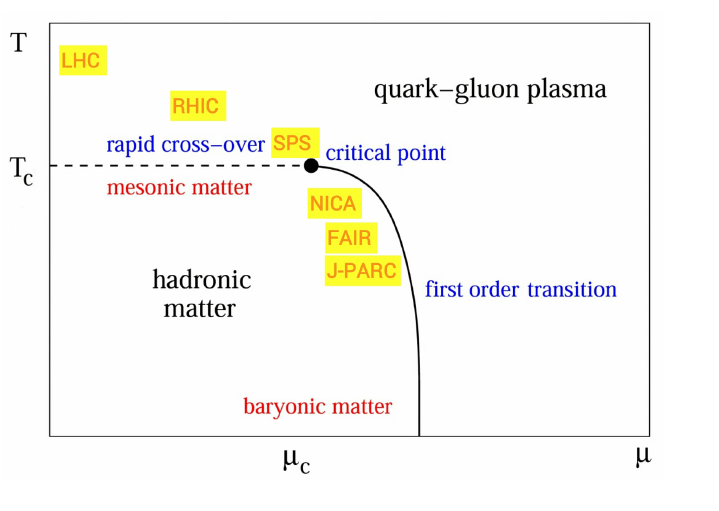
\includegraphics[width=1.\linewidth]{corr_femto5.png}
      \end{figure}
    \end{block}
    \column{.48\textwidth}
    \begin{block}{\center \bf \alert{The Questions arisen:}}
      {\bf 
       \begin{itemize}
   %    \item 1st order phase transition (PT) to the QGP occurs at lower energies(?)
       \item At what energies do the hydro models with the 1st order phase transition (1PT) describe femtoscopy observables better than those
         with crossover?
       \item What femtoscopy observables are the most sensitive to this difference?
       \end{itemize}
       }
     \end{block}
  \end{columns}
  \note{
    { \tiny
      The performed experiments at RHIC and LHC clearly demonstrate that hot and dense
      matter with the partonic collectivity is formed in the ultra-relativistic
      heavy-ion collisions at large $\sqrt{s_{NN}}$. 
      The observed effects (jet quenching, charmonium suppression,
      strangeness enhancement etc.) are considered to be the signals of
      a transition to the deconfined phase.
      The regime obtained in heavy ion collisions at the highest RHIC energies seems to correspond to lattice QCD calculations
      for a rapid, smooth crossover at large temperature T and vanishing baryonic chemical potential $\mu_{B}$.
      Various models predict a strong 1st order transition at low temperatures and large $\mu_{B}$.
      One may thus expect the ``critical point `` (CP) in the QCD phase diagram.
      The existing numerical techniques in lattice QCD calculations meet difficulties for $\mu_{B}$ > 0 thus leading to
      theoretical uncertainties in the prediction of the location of the critical point.
      The modern market of Monte Carlo generators has many well developed hydro models that could be applicated to this issue.
      Therefore, in sense of femtoscopy, the following questions become important (see the Slide).   
    }
  }
\end{frame}

\begin{frame}
  \frametitle{Femtoscopy: Energy Scan}
  \begin{columns}
    \column{.48\textwidth}
    \begin{block}{}
      \footnotesize{
        \begin{center}
          \bf
          RHIC: $\sqrt{s_{NN}}$ = 62 to 200 GeV
          
          \vspace{0.15cm}
          
          \alert {large T \& small $\mu_{B}$}

          \vspace{0.15cm}
          
          % {\tiny New state of matter, the strongly coupled Quark Gluon Plasma (sQGP)}

          \vspace{0.15cm}
          
          \alert {Smooth, rapid crossover}

        \end{center}
      }
    \end{block}
    
    \begin{block}{}
      \footnotesize{
        \begin{center}
          \bf
         BES @ RHIC: $\sqrt{s_{NN}}$ = 7.7, 11.5, 19.6, 27, 39 GeV

        \vspace{0.2cm}
        
        \alert {small T \& large $\mu_{B}$}

        \vspace{0.15cm}
        
       % {\tiny search for ``critical point''}

        \vspace{0.15cm}
      
        %\alert {1st order phase transition}
        \alert{search for ``critical point''}
         \end{center}
      }
    \end{block}
    \begin{block}{}
      \footnotesize{
        \begin{center}
          \bf
          NICA: $\sqrt{s_{NN}}$ = 4 to 11 GeV

           \vspace{0.15cm}
        
           \alert {small T \& large $\mu_{B}$}

        \end{center} 
      }
    \end{block}
   
    \column{.48\textwidth}
    \begin{block}{\center \tiny \bf STAR, Phys.Rev. C92 (2015) 1, 014904}
      \begin{figure}[H]
        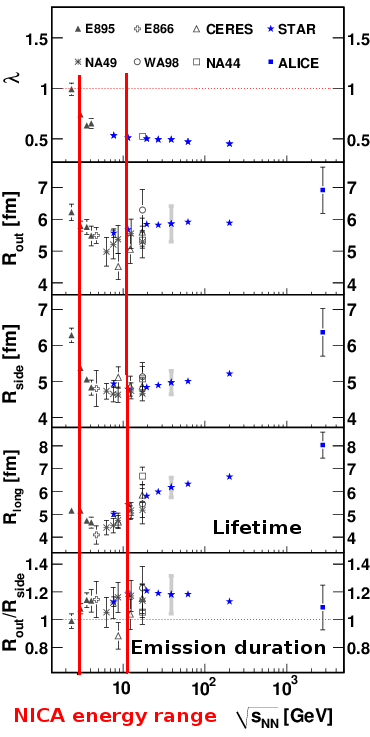
\includegraphics[width=.6\linewidth]{RiRootS.png}
      \end{figure}
    \end{block}
  \end{columns}
  \note{
    %The heavy-ion collisions at the highest RHIC energies are described
    % using the lattice QCD calculations  
    %assuming a crossover transition at high temperature T and
    %vanishing baryonic chemical potential 
    %$\mu_B$. At the same time, there are models that predict a strong first order
    %phase transition at moderate temperatures and large $\mu_B$,
    %which takes place at moderate and low energies.
    

    Therefore, the NICA complex operating in the energy region
    $\sqrt{s_{NN}}$ = 4 -- 11 GeV is suitable for the critical point location
    search via experimental detection of its signatures. 
  }
\end{frame}

\begin{frame}
  \frametitle{Expected features of the 1st order PT}
  \begin{columns}[c]
    \column{.48\textwidth}
    \begin{block}{}
     {\footnotesize \bf 1PT: $R_{out} / R_{side} >> 1$ \& large $R_{long}$ due to emission stalling during PT}
    \end{block}
    \begin{block}{\center \footnotesize \bf D. H. Rischke and M. Gyulassy,  Nucl. Phys. A608, 479 (1996)}
      \begin{figure}[H]
        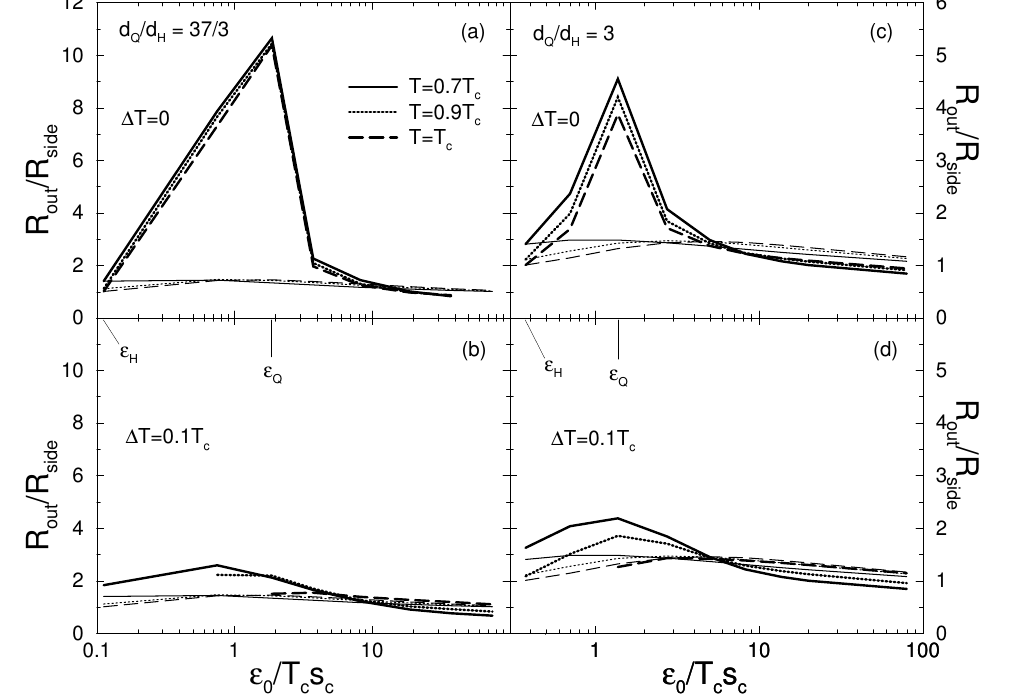
\includegraphics[width=0.75\linewidth]{corr_femto6.png}
      \end{figure}
 %     {\tiny r-t correlations in expanding source reduce the observed $R_{out}$ $\rightarrow$ $R_{out} / R_{side}$} 
    \end{block}
    \begin{block}{}
      {\centering \footnotesize \bf \alert {What do the modern  hydrodynamic (hybrid) models expect?}}
    \end{block}
    \column{.48\textwidth}
    \begin{block}{\center \tiny \bf STAR, Phys.Rev. C92 (2015) 1, 014904}
      \begin{figure}[H]
        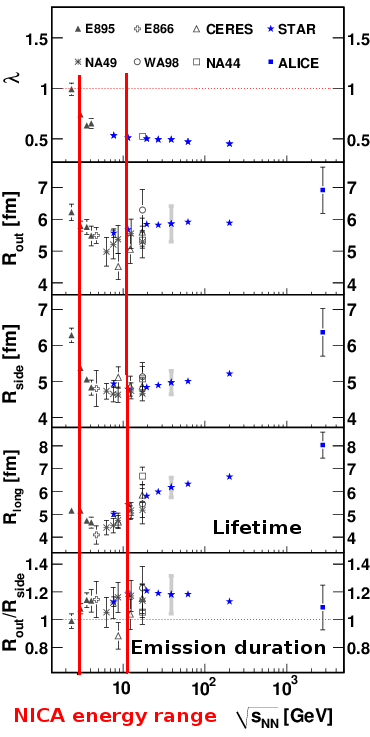
\includegraphics[width=.6\linewidth]{RiRootS.png}
      \end{figure}
    \end{block}
  \end{columns}
  \note{
    { \tiny
      Study of femtoscopic correlations allows one to constrain the model
      predictions for an early stage of collision and fireball evolution.
      It was expected that the first order phase transition strongly delays
      the fireball evolution, but the pion correlation radii
      measured in a wide energy range (from the AGS to the RHIC energies)
      demonstrated a weak energy dependence and didn't reveal the expected behavior for the phase
      transition. The weak energy dependence of femtoscopic
      radii in the AGS-SPS-RHIC energy region and the
      overestimation of these radii by various transport and hydrodynamic models was considered
      as a femtoscopy puzzle.
      This puzzle motivated a development of more sofisticated
      hydrodynamic models allowing for a simultaneous description
      of single particle and correlation observables, including
      the femtoscopic ones. According to them, the femtoscopic radii, particle spectra and
      elliptic flow can be described using the initial Gaussian density profile
      and by including a combination of several effects: pre-thermal acceleration,
      a stiffer EoS and adding viscous corrections.
      Therefore, we arrive at the main question: What do the modern  hydrodynamic (hybrid) models expect? 
    }
  }
\end{frame}

\begin{frame}
  \frametitle{Search for critical point location}
  \begin{columns}
    \column{.48\textwidth}
    \begin{block}{\bf \centering Softening? Critical point?}
      \begin{figure}[H]
        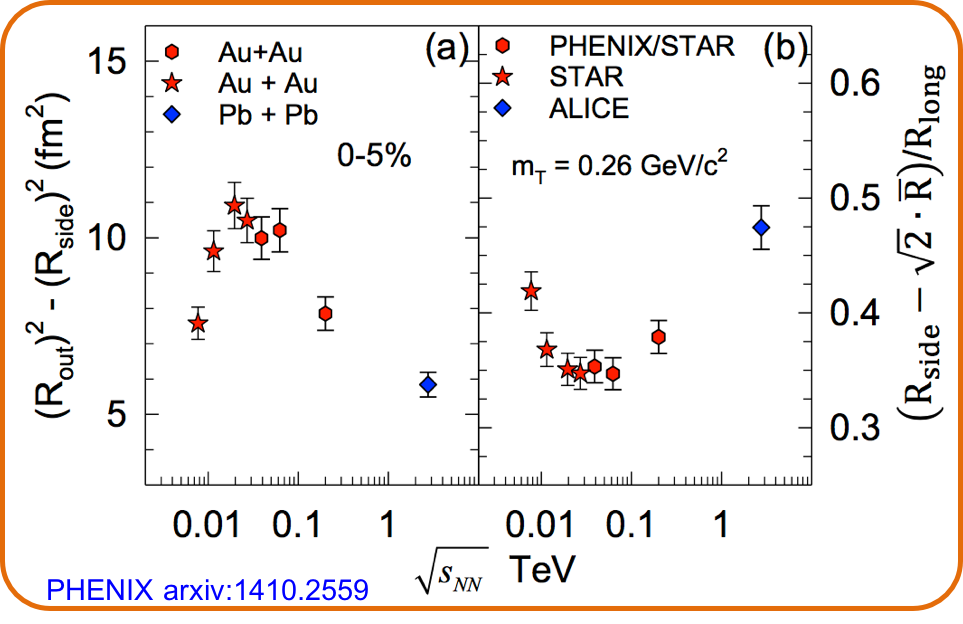
\includegraphics[width=.8\linewidth]{Rout2Rside2.png}
      \end{figure}
    \end{block}
    \column{.48\textwidth}
    \begin{block}{}
       \begin{figure}[H]
        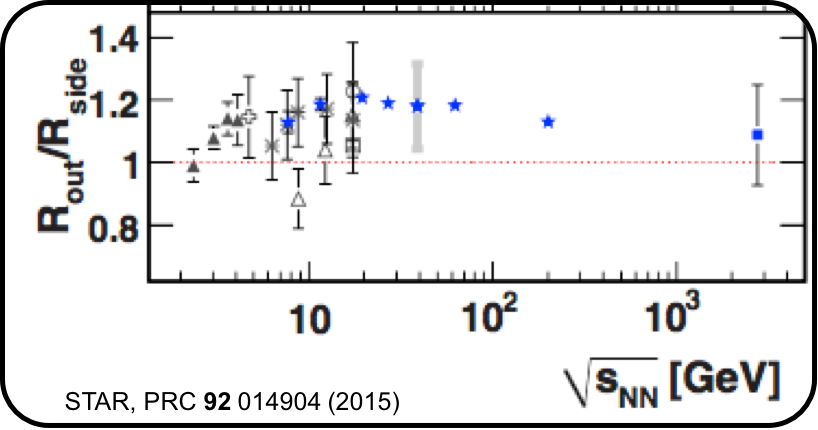
\includegraphics[width=.9\linewidth]{RoutRside_scale.png}
      \end{figure}
    \end{block}
  \end{columns}
  
  \begin{block}{ \bf \centering Mike Lisa, QM 2015:}
    \bf
    {\color{red} This is precisely the sort of thing we’ve been seeking, \& it’s happening in ``interesting'' BES energies.
    It requires and deserves serious theory / modeling.}
  \end{block}
\end{frame}

\begin{frame}[shrink=60]
  \frametitle{vHLLE + UrQMD model}
   \begin{block}{{ \bf Iu. Karpenko, P. Huovinen, H.Petersen, M. Bleicher, Phys.Rev. C 91, 064901 (2015) \\
    vHLLE code: free and open source, https://github.com/yukarpenko/vhlle}}
    \begin{figure}[H]
      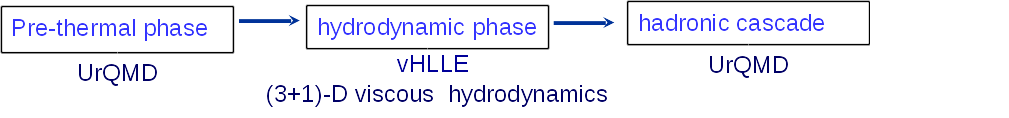
\includegraphics[width=.8\linewidth]{vHLLE.png}
    \end{figure}
  \end{block}
  \begin{columns}[c]
    \column{.48\textwidth}
     \begin{block}{}
       { \bf \center Chiral EoS - \alert{crossover} \\}
       { \bf J. Steinheimer et al, J. Phys. G 38, 035001 (2011)}
     \end{block}
     \column{.48\textwidth}
      \begin{block}{}
        {\bf \center HadronGas + Bag Model - \alert{1PT} \\}
        { \bf P. F. Kolb et al, Phys.Rev. C 62, 054909 (2000)}
     \end{block}
  \end{columns}
  \begin{block}{}
    \begin{figure}[H]
      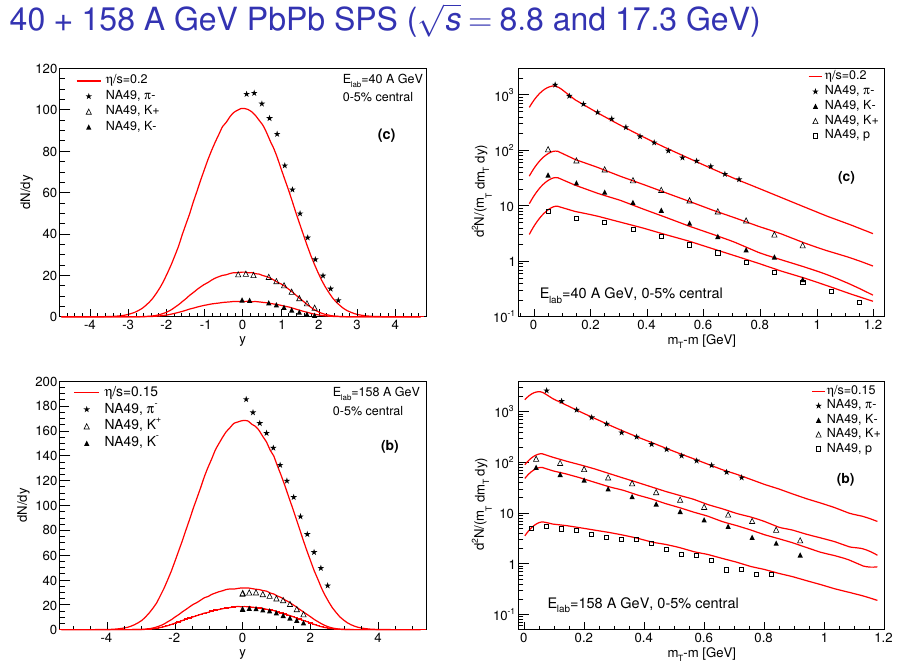
\includegraphics[width=.6\linewidth]{vhlle_calibr.png}
    \end{figure}
  \end{block}
   \note{
     In order to answer this question the hybrid vHLLE + UrQMD model was chosen as a candidate
     to clarify the situation. It is an open source well documented code that can be downloaded for usage.
     The model description is given in this reference.
     Of course, many thanks to Yu.~Karpenko for his fruitful advices and discussions we had together.
     We tried to use other models having an opportunity to include hydro phase in the calculations (like pure UrQMD, for example),
     but it didn't describe well the available experimental data.
     Therefore, it is required to have a model that describes on a reasonable level the experimental data.
     The chosen candidate is tuned with the existing experimenatal data.
     The results obtained are in a good agreement with the
     experimental ones.
   }
\end{frame}

\begin{frame}[shrink=20]
  \frametitle{vHLLE + UrQMD model}
  \begin{block}{{ \bf {\footnotesize Iu. Karpenko, P. Huovinen, H.Petersen, M. Bleicher, Phys.Rev. C 91, 064901 (2015)} \\
    vHLLE code: free and open source, https://github.com/yukarpenko/vhlle}}
    \begin{figure}[H]
      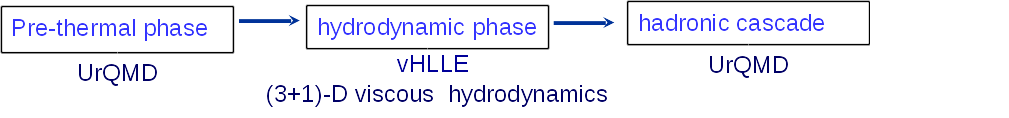
\includegraphics[width=.8\linewidth]{vHLLE.png}
    \end{figure}
  \end{block}
  \begin{columns}[c]
    \column{.48\textwidth}
        \begin{block}{\center \footnotesize \bf \alert{vHLLE}}
        \begin{figure}[H]
          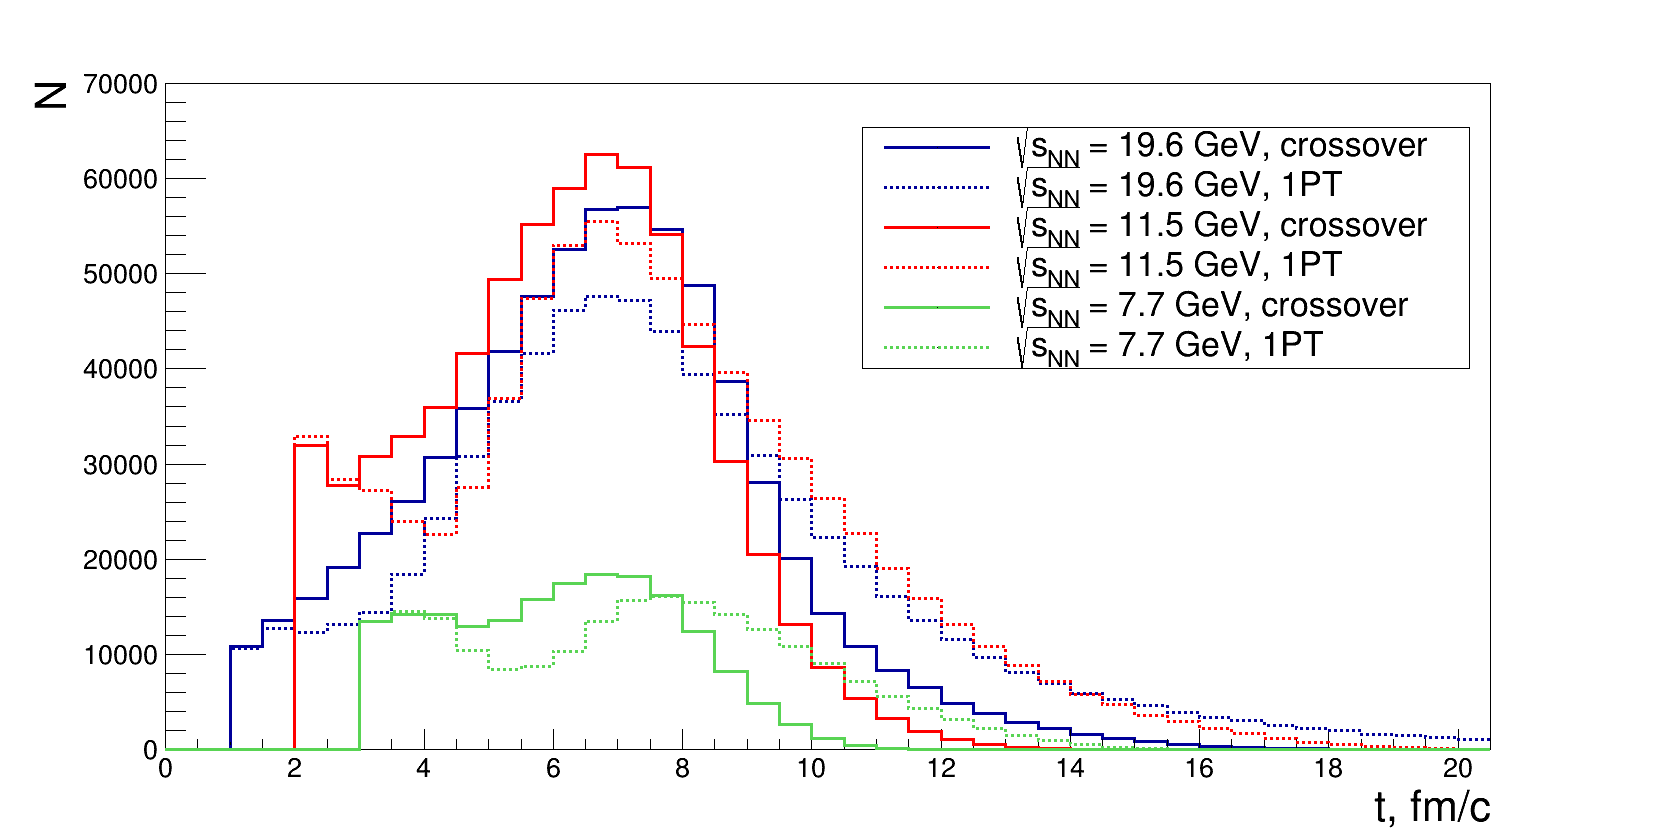
\includegraphics[width=.95\linewidth]{vHLLE_tfr.png}
        \end{figure}
     \end{block}
     \column{.48\textwidth}
         \begin{block}{\center \footnotesize \bf \alert{vHLLE + UrQMD}}
        \begin{figure}[H]
          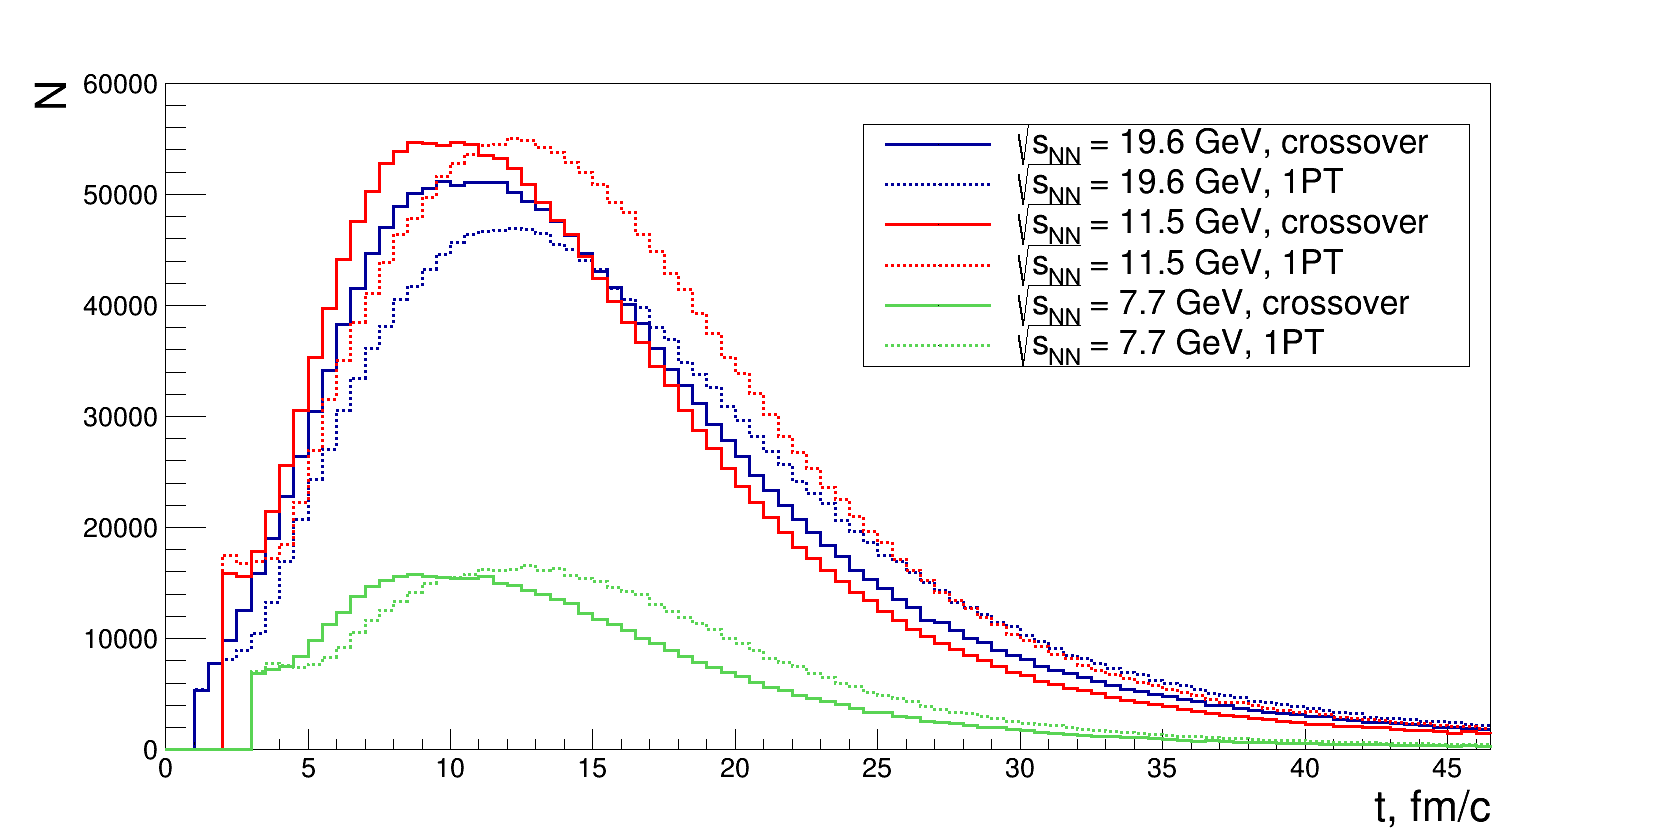
\includegraphics[width=.95\linewidth]{vHLLE_UrQMD_tfr.png}
        \end{figure}
     \end{block}
  \end{columns}
    \begin{block}{}
    \bf \centering 
        {\color{red} Hydro phase lasts longer with 1PT, especially at lower energies
          but cascade smears this difference}.
        
        Is it possible to see this time difference using the femtoscopy techniques?
    \end{block}
   
\end{frame}


\begin{frame}[shrink=50]
  \frametitle{Radii versus $k_{T}$ with the vHLLE + UrQMD model}
  \begin{columns}
    \column{.20\textwidth}
    \column{.60\textwidth}
    \begin{block}{\bf \centering Details of analysis}
     \bf \centering 
      vHLLE + UrQMD: $\sim$ 100 000 events,
      $\pi^{+}\pi^{+}$ pairs,     
      0.15 $ < p_{T} < $ 0.8 GeV/c,      
      $|\eta| < 1$,      
      $k_{T}$ bins (in GeV/c): $[0.15, 0.25]$, $[0.25, 0.35]$, $[0.35, 0.45]$, $[0.45, 0.60]$
      
    \end{block}
    \column{.20\textwidth}
  \end{columns}
  
  \begin{columns}
    \column{.48\textwidth}
    \begin{block}{\bf \centering AuAu @ $\sqrt{s_{NN}} = 7.7$ GeV}
       \begin{figure}[H]
         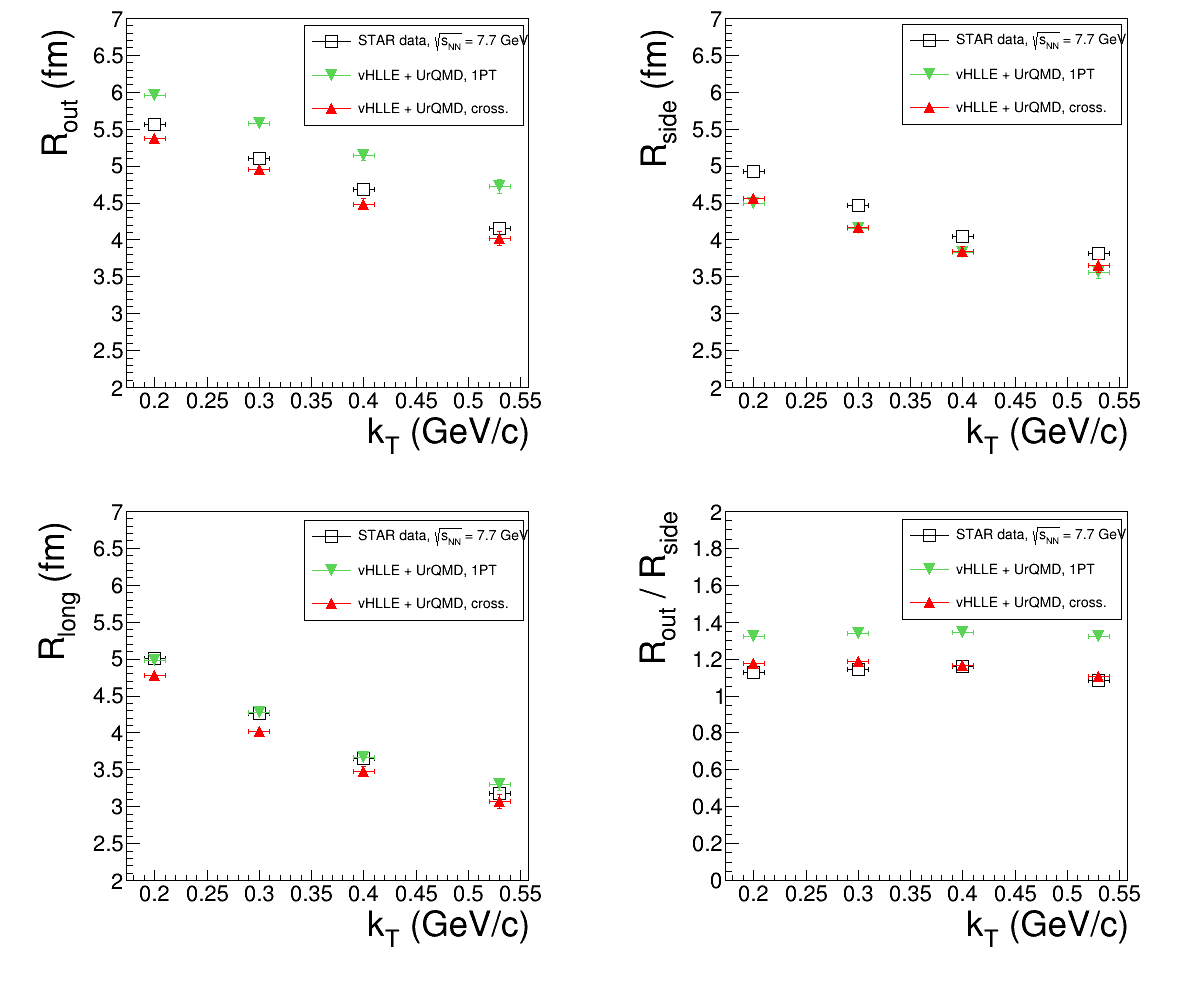
\includegraphics[width=.95\linewidth]{radii_077gev_STAR_vs_kT.png}
       \end{figure}
    \end{block}
    \column{.48\textwidth}
    \begin{block}{\bf \centering AuAu @ $\sqrt{s_{NN}} = 11.5$ GeV}
       \begin{figure}[H]
         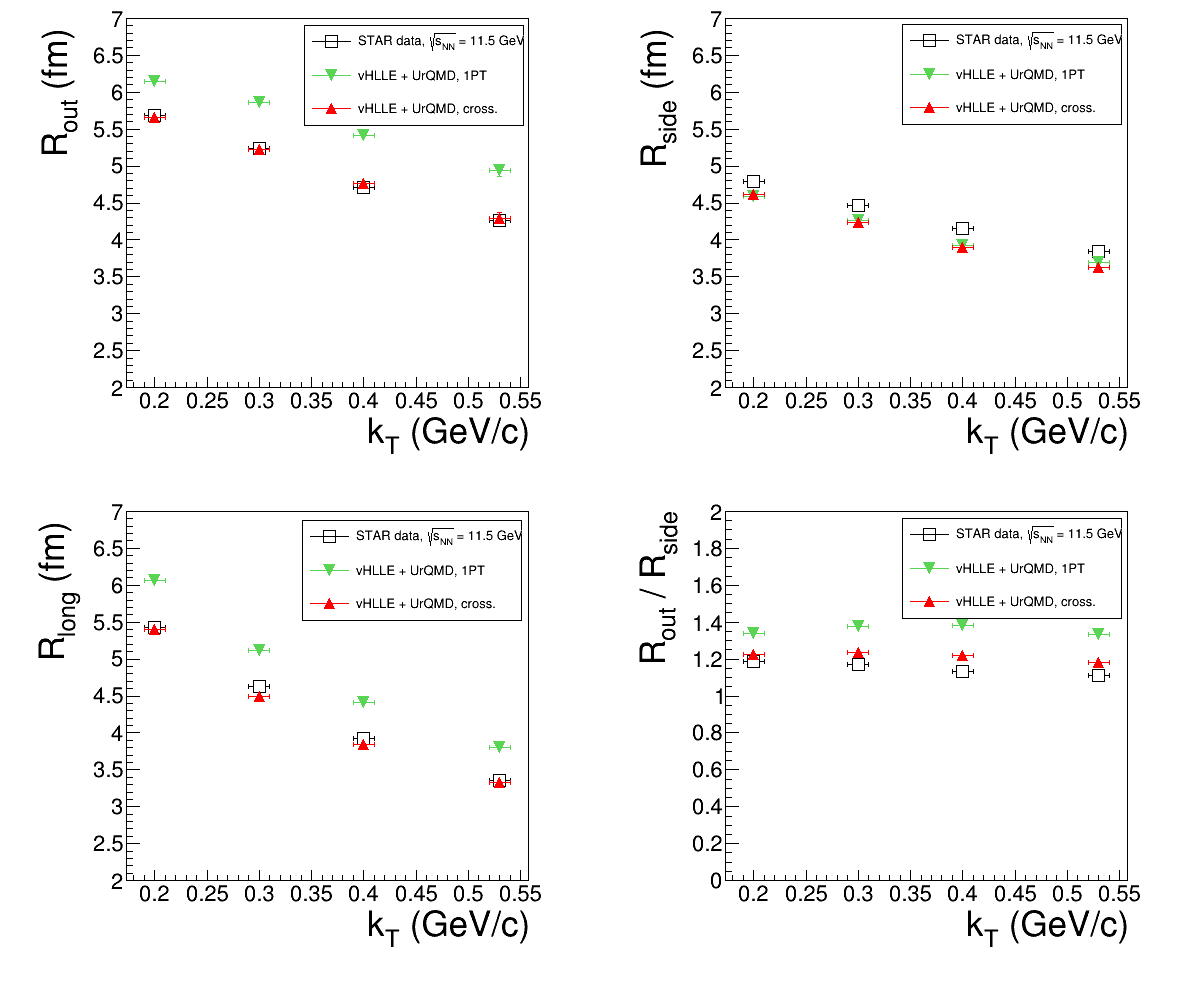
\includegraphics[width=.95\linewidth]{radii_115gev_STAR_vs_kT.png}
       \end{figure}
    \end{block}
  \end{columns}
  \begin{columns}
    \column{.20\textwidth}
    \column{.60\textwidth}
    \begin{block}{}
      \bf 
      \begin{itemize}
      \item $R_{long}$ (1PT) > $R_{long}$ (crossover), difference $\sim$ 0.5 fm
        \vspace{0.2cm}
      \item $R_{out}/R_{side}$ (1PT) > $R_{out} / R_{side}$ (crossover)
      \end{itemize}
%      \vspace{0.2cm}
 %     It seems that $vHLLE + UrQMD$ model with crossover describes the STAR data
 %     better than the one with the 1PT.
 %     \vspace{0.2cm}
      \begin{center}
        {\bf {\color{red} A more detailed study is required ...}}
      \end{center}
    \end{block}
    \column{.20\textwidth}
  \end{columns}
  \note{
    As a first test, using the model, it was initiated an attempt to reproduce the 3D femtoscopy radii obtained
    by the STAR collaboration at two values of $\sqrt{s_{NN}}$. Detailes of the analysis are presented in the slide.
    The experimental data are presented by empty squares. The model calculations using the EoS assuming the 1st order phase transition
    are presented by green triangles, meanwhile, the calculations with the EoS of croosover type -- by red triangles.
    It possible to see that the experimental data are described better with the simulations assuming crossover.
    $R_{long}$ that is sensitive to freeze-out time of system is overestimated by the EoS with 1PT.
    Also the ratio $R_{out} / R_{side}$ sensitive to emission duration is better described by the EoS with crossover. 
  }
\end{frame}

\begin{frame}[shrink=10]
  \frametitle{Source Function Technique}
  \begin{columns}
    \column{.48\textwidth}
    \begin{block}{}
      $S(r^{*})$ is a {\bf source function}, which represents time-integrated distribution of particle emission points separation
      $r^{*}$ in the PRF.
    \end{block}
     \begin{block}{}
       $C({\bf q}) - 1 \equiv R({\bf q}) = \int (|\phi({\bf q, r})|^{2} - 1) S({\bf r}) d{\bf r}$
     \end{block}
      \begin{block}{}
        The method is suitable for extracting the $S(r^{*})$ directly from the data {\bf {\color{red}without any hypothesis about source shape}}.
       
    \end{block}
    \column{.48\textwidth}
     \begin{block}{\centering {\tiny \bf STAR, Phys.Rev. C88 (2013) 3, 034906}}
       \begin{figure}[H]
         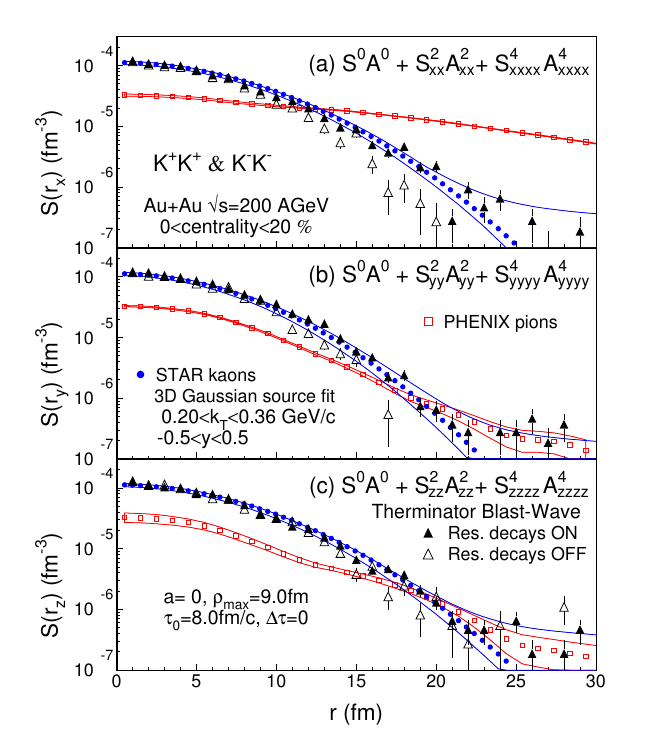
\includegraphics[width=.95\linewidth]{source_func.png}
       \end{figure}
     \end{block}
  \end{columns}
  \note{%The PHENIX and STAR collaborations applied a ``new imaging technique'' to extract ...
    %\\
    %It seems to be very useful for comparison of the experimental data with the models with the 1PT or crossover EoS.
    To obtain a more detailed information on the space-time structure
    of the system, as compared with that in Gaussian correlation radii,
    one use more complicated parametrizations accounting for non-Gaussian
    tails, or exploit the source imaging technique. The latter
    is based on Fourier-like extraction of the emission function from the
    measured correlation function in the PRF; being formally
    model-independent, it is however quite unstable thus requiring still
    some stabilizing model assumptions.
    In case of an arbitrary (non-Gaussian) source function, using this technique,
    it is possible to see the detailed source structure, which can
    likely deviate from the Gaussian distribution, having a more complicated shape.
    It is caused by different reasons, such as collision geometry,
    contribution of long-lived resonances, space-momentum correlations, etc.
    So, the source imaging gives a real possibility to study an influence of
    these effects on the source form.
}
\end{frame}

\begin{frame}[shrink=50]
  \frametitle{Source Function Technique}
  \begin{columns}
    \column{.20\textwidth}
    \column{.60\textwidth}
    \begin{block}{\bf \centering Details of analysis}
      \bf \centering 
      vHLLE + UrQMD: a very first test.
      
      $\pi^{+}\pi^{+}$ pairs,       
      0.15 $ < p_{T} < $ 0.8 GeV/c, 
      $|\eta| < 0.5$,
      $k_{T}$ bins (in GeV/c): $[0.2, 0.4]$
      
    \end{block}
    \column{.20\textwidth}
  \end{columns}
  \begin{columns}
    \column{.48\textwidth}
    \begin{block}{\bf  \centering $\sqrt{s_{NN}} = 7.7$ GeV, vHLLE}
      \begin{figure}[H]
         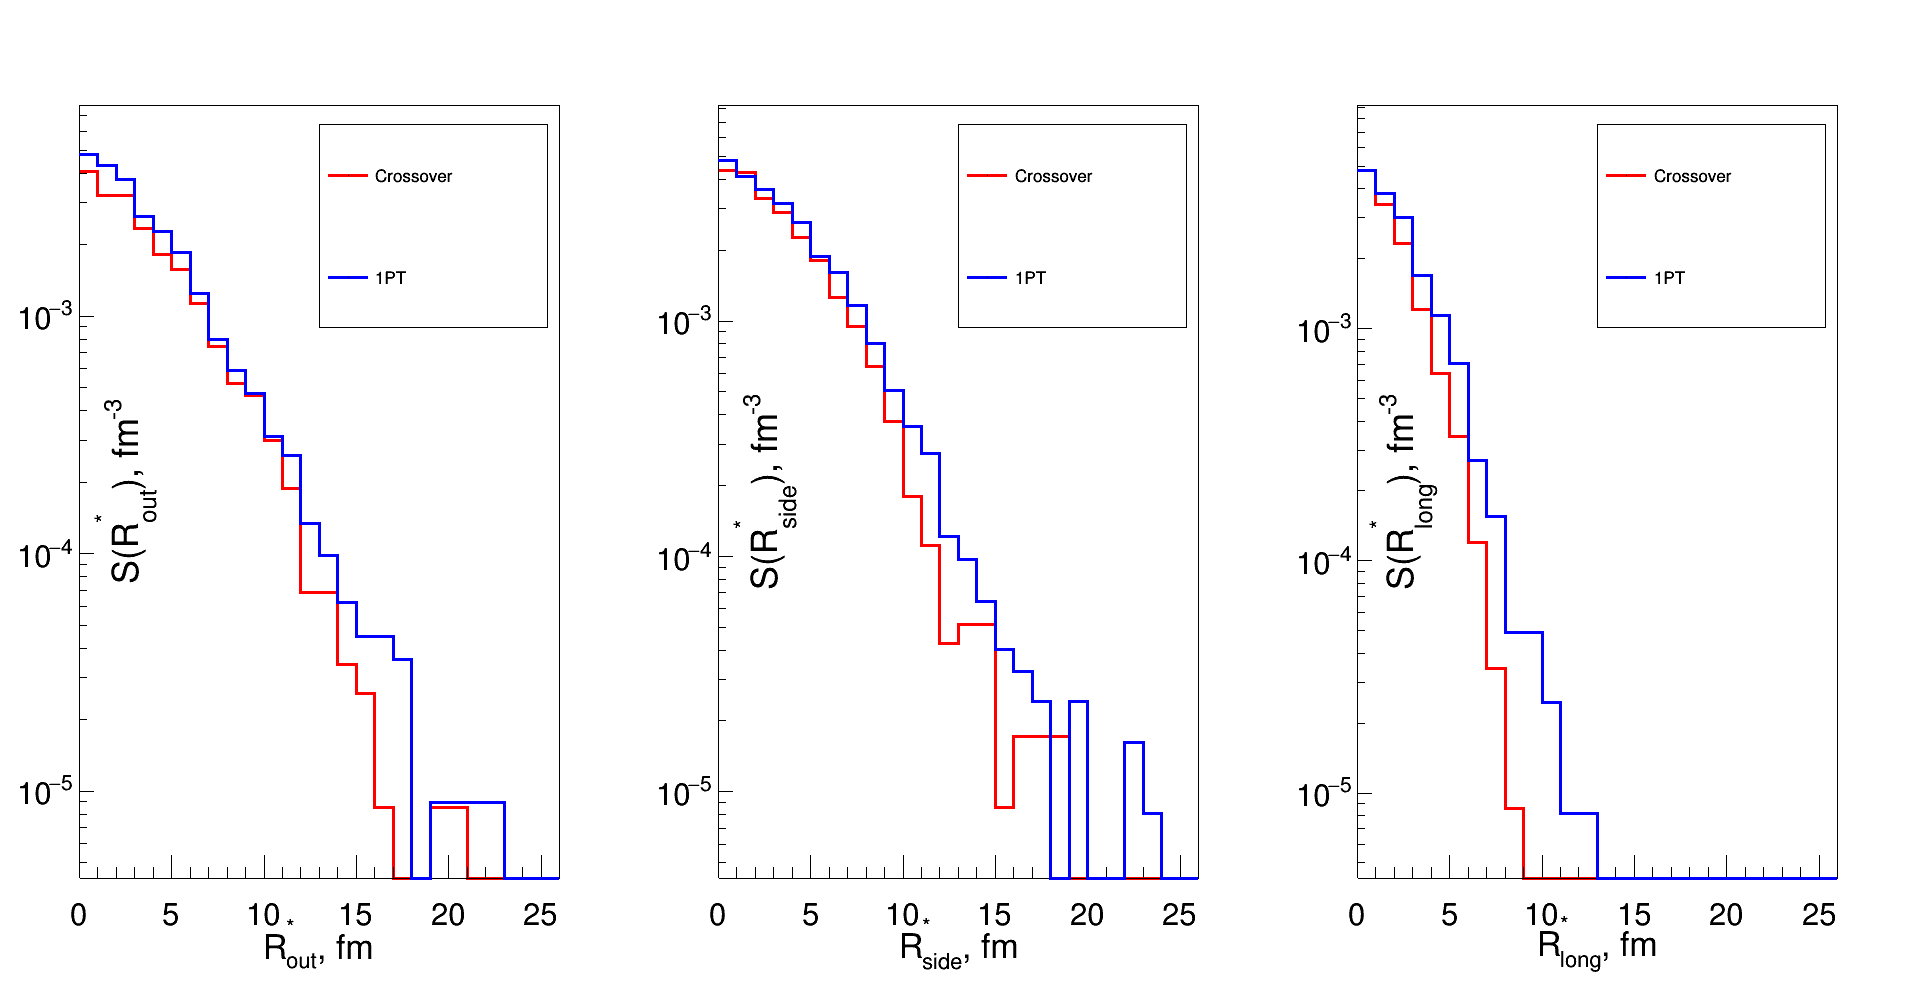
\includegraphics[width=.95\linewidth]{SF_vHLLE_77gev.png}
      \end{figure}
    \end{block}
    \begin{block}{\bf  \centering $\sqrt{s_{NN}} = 7.7$ GeV, vHLLE + UrQMD}
      \begin{figure}[H]
        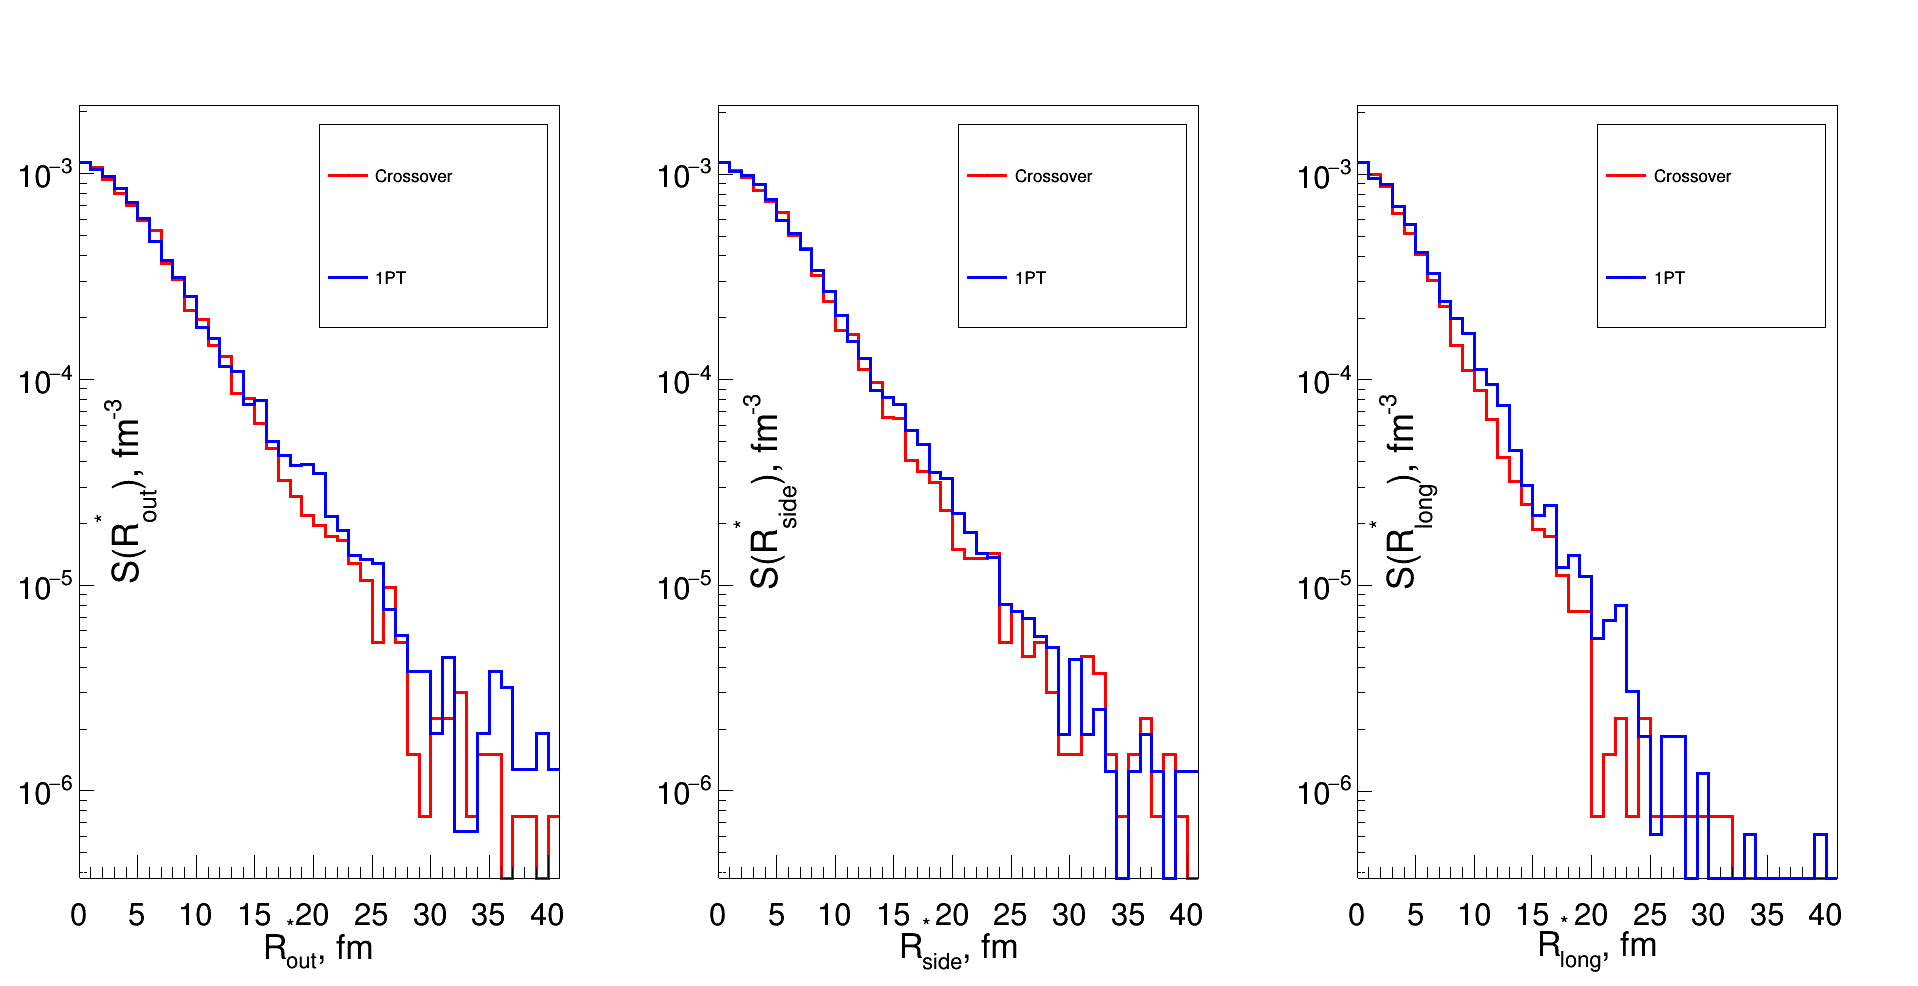
\includegraphics[width=.95\linewidth]{SF_vHLLE_UrQMD_77gev.png} \\
      \end{figure}
    \end{block}
    \column{.48\textwidth}
     \begin{block}{\bf \centering $\sqrt{s_{NN}} = 11.5$ GeV, vHLLE}
       \begin{figure}[H]
         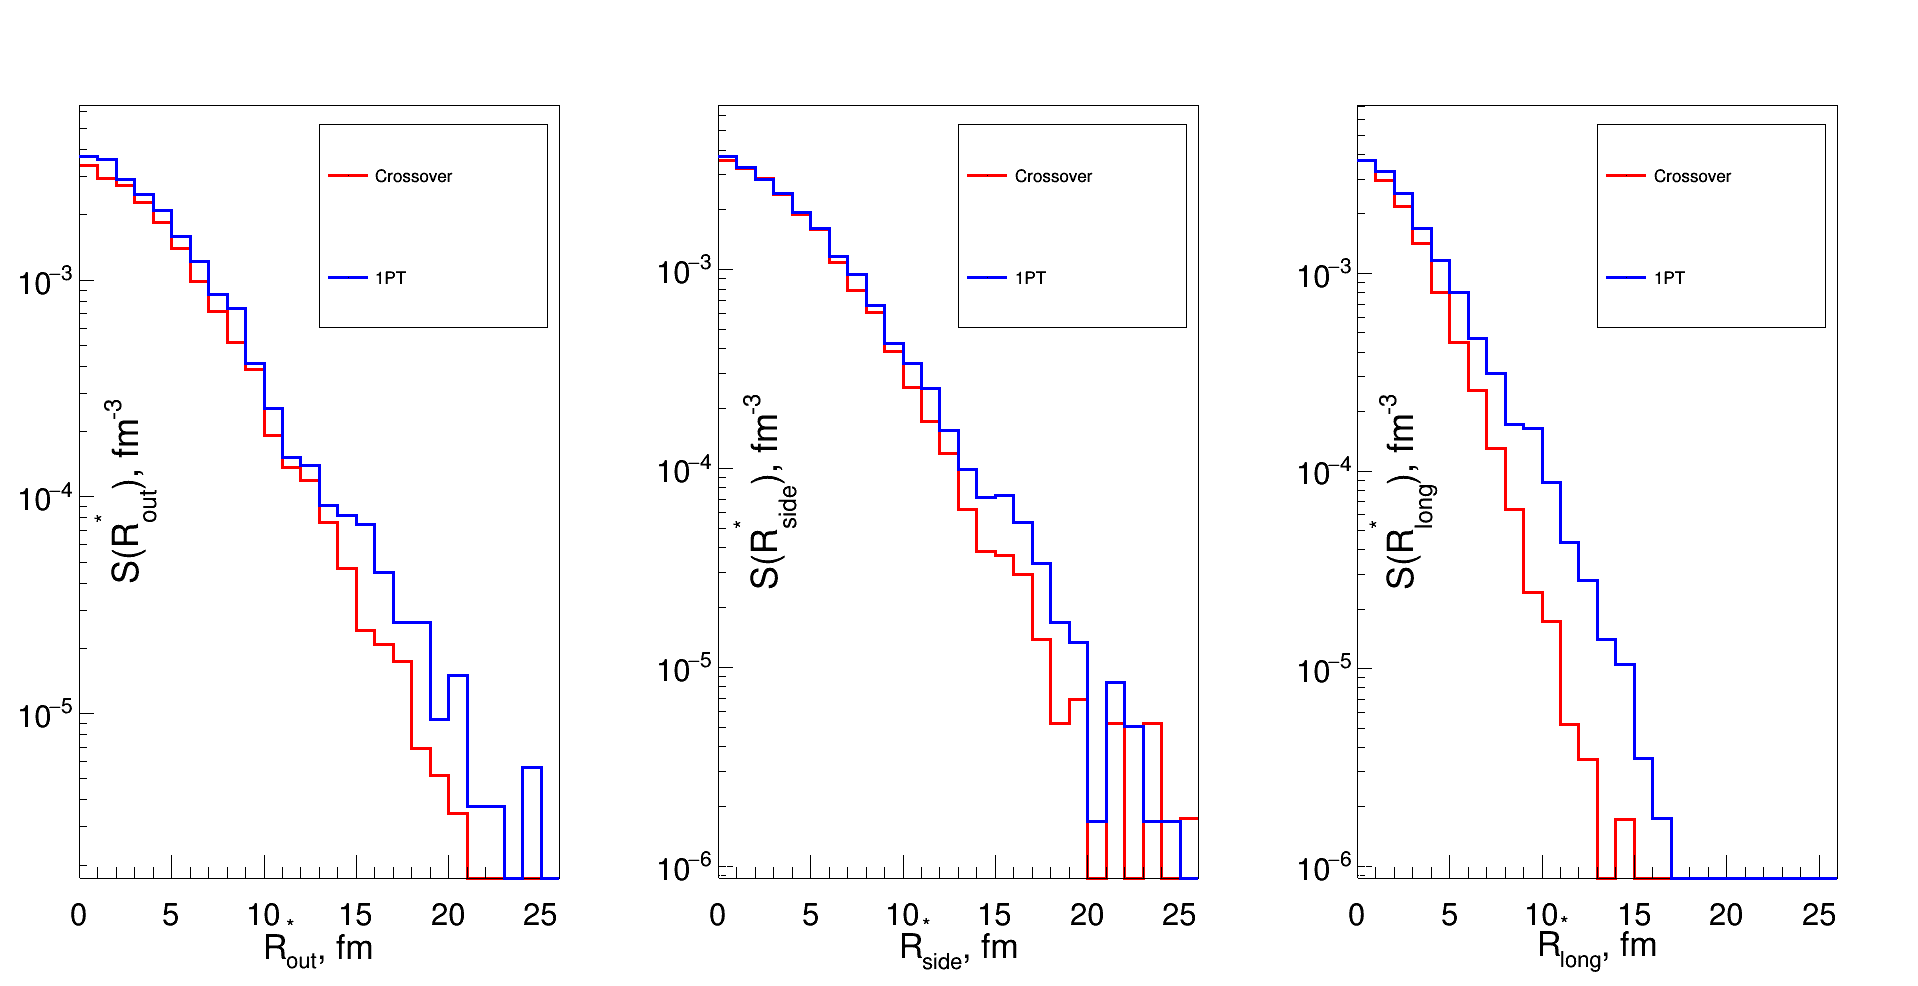
\includegraphics[width=.95\linewidth]{SF_vHLLE_115gev.png}
       \end{figure}
    \end{block}
    \begin{block}{\bf \centering $\sqrt{s_{NN}} = 11.5$ GeV, vHLLE + UrQMD}
      \begin{figure}[H]
         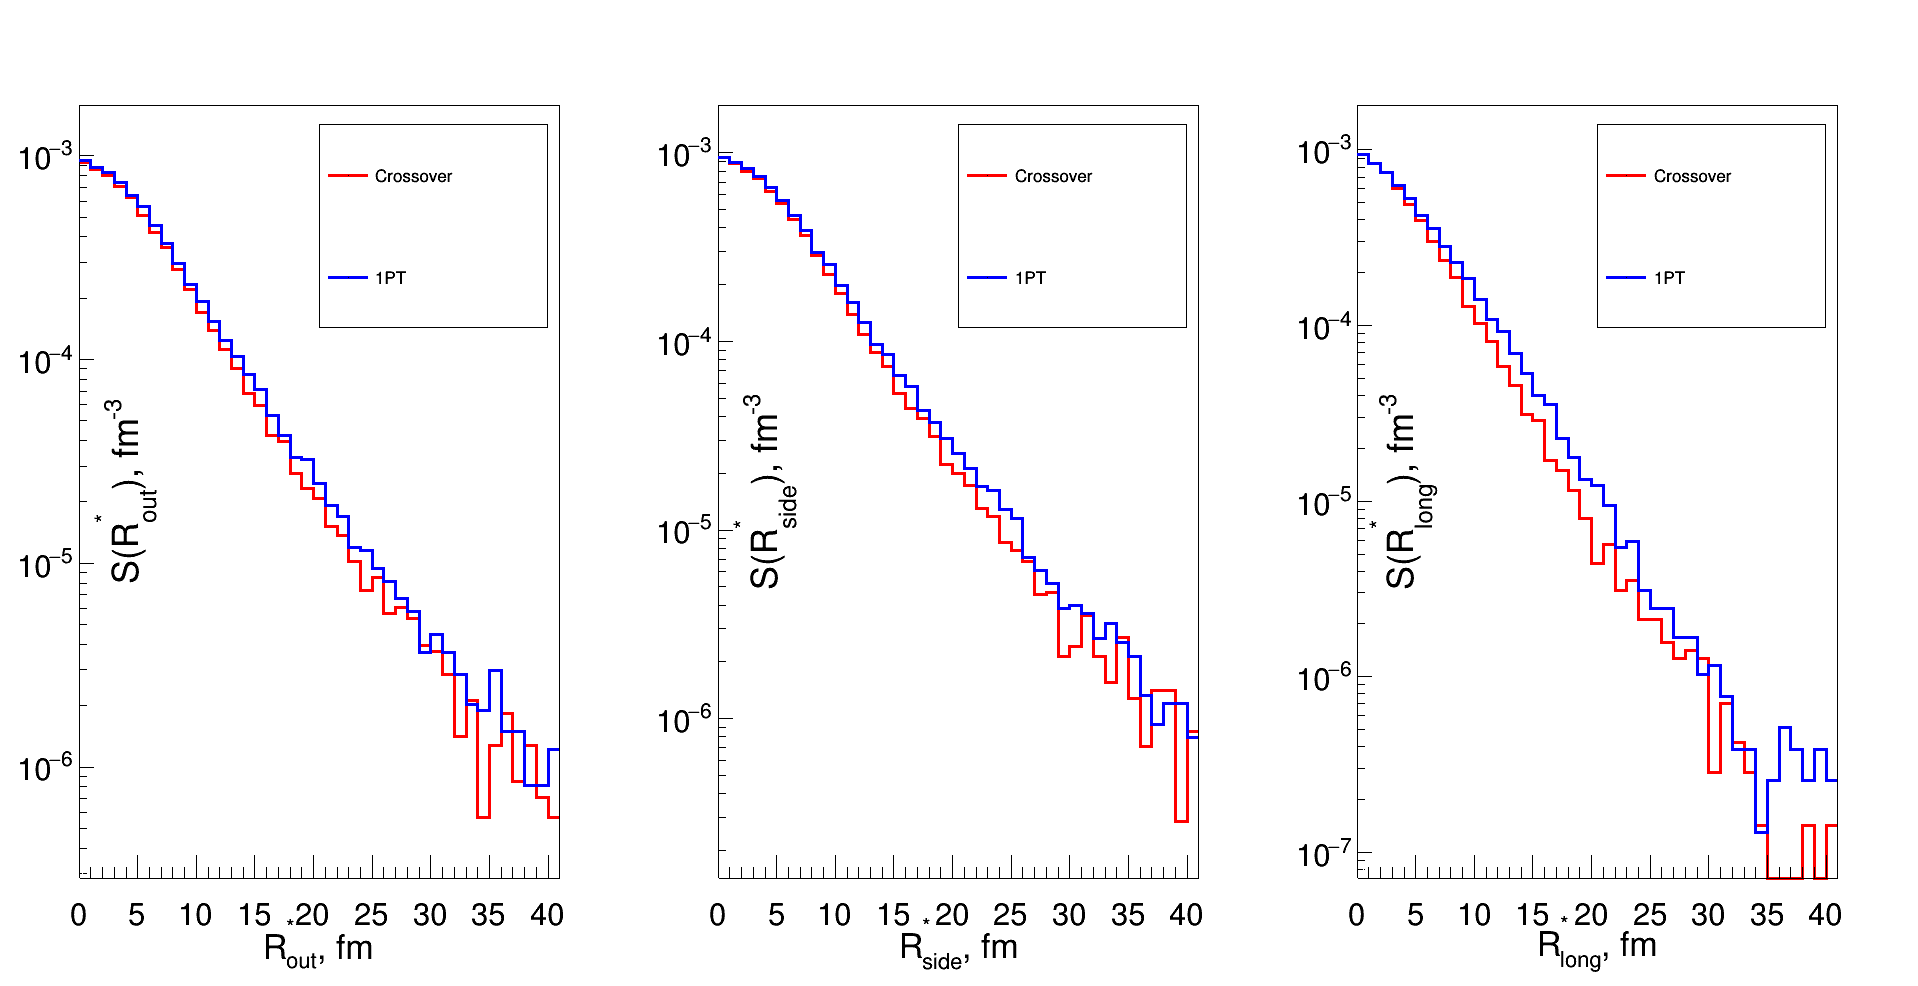
\includegraphics[width=.95\linewidth]{SF_vHLLE_UrQMD_115gev.png}
      \end{figure}
    \end{block}
  \end{columns}
  \note{
    In the slide projections of the source function in the PRF on 
    out, side and longitudinal directions are presented.
    The source function was obtained for pions at different
    $\sqrt{s_{NN}}$ using the vHLLE+UrQMD model.
    It was established, that the source function is not very sensitive to
    $k_{T}$ and, due to this fact, the pion pairs used in the analysis
    satisfy the condition $0.2 \leq k_{T} \leq 0.4$ GeV/c. Also,
    there was applied a cut on pseudorapidity ($|\eta| < 0.5$).
    One may see that for calculations with the first order phase
    transition the visible tails of the source function are longer than those
    obtained using crossover.
    The largest difference is seen in the longitudinal direction,
    the effect becoming more visible with the increasing energy.
    The search for anomalous non-Gaussian tails is motivated
    by the fact that the onset of the first order phase transition
    should slow down the fireball expansion thus leading to
    an increase of its evolution (freeze-out) time. 
  }
\end{frame}

\begin{frame}
  \frametitle{Conclusion, Part 1}
  \bf \centering 
  \begin{itemize}
  \item Despite hadronic cascade affects strongly the observed source functions, it seems to be possible to distinguish them within the vHLLE + UrQMD hybrid model.
  \item Hydro phase lasts longer with the 1PT.  
  \item We plan to continue these studies with larger statistics for $\pi$- and $K$-mesons.
  \item The vHLLE + UrQMD model with crossover describes the RHIC femtoscopy radii at $\sqrt{s_{NN}}$  = 7.7, 11.5 GeV
    better than with the 1PT. 
  \item $R_{long}$ (1PT) $ > $ $R_{long}$ (crossover),  the observed difference is rather small for low energies. 
  \item $R_{out} / R_{side}$ (1PT) $ > $ $R_{out} / R_{side}$ (crossover), the observed difference is rather small for low energies. 
  \item We plan to study the non-Gaussian tails of CFs using different parametrizations: e.g. Hump or Edgeworth parametrizations.
  \end{itemize}
\end{frame}

\begin{frame}
  \frametitle{}
  \bf \centering {\color{red} Thank you for your attention!}
\end{frame}


\begin{frame}
  \bf \centering {\color{blue} BACKUP SLIDES}
\end{frame}

\begin{frame}
  \frametitle{Splitting and Merging effects}
  \begin{block}{}
 \begin{figure}[H]
     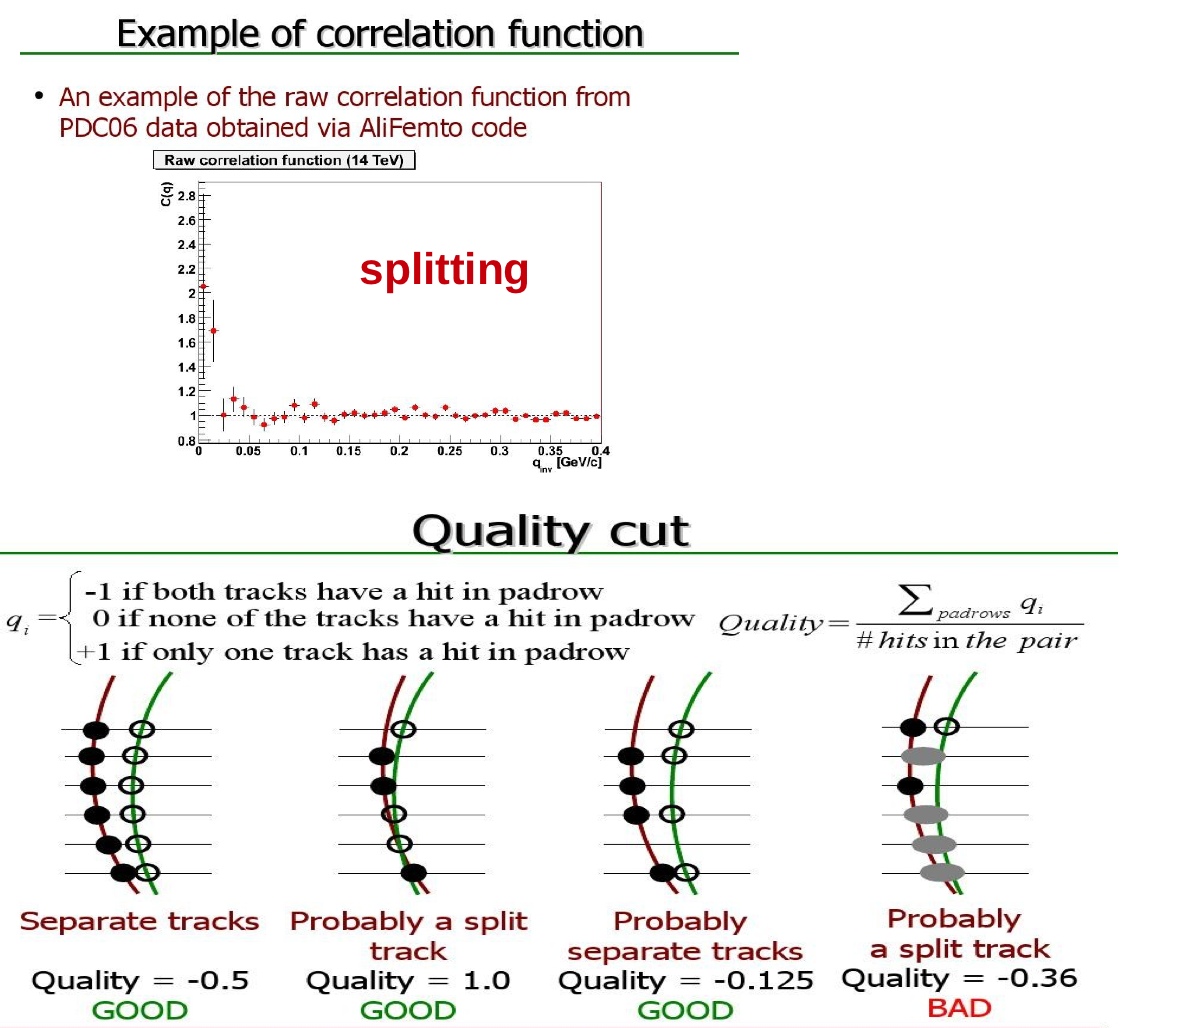
\includegraphics[width=.70\linewidth]{splitting_demo.png}
   \end{figure}
  \end{block}
\end{frame}

\begin{frame}
  \frametitle{Anti-merging cut (The ALICE collaboration)}
  \begin{block}{}
    \begin{figure}[H]
      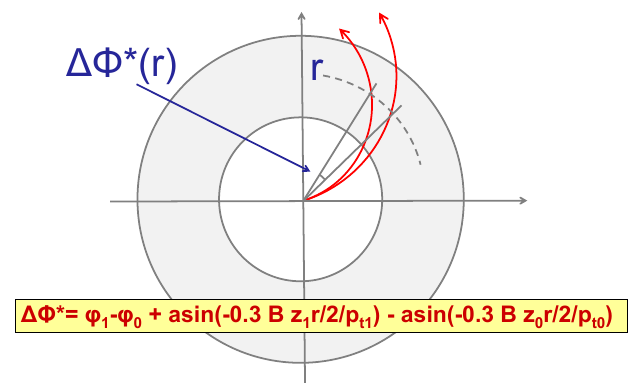
\includegraphics[width=.45\linewidth]{PhiStar.png}
    \end{figure}
  \end{block}
  \begin{block}{}
    \bf \centering 
    \begin{equation*}
      \Delta \Phi^{*}(R) = \phi_{1} - \phi_{0} + \arcsin \left(-\dfrac{0.3 B_{z} Z_{1} R}{2 P_{T1}}\right) - \arcsin \left(-\dfrac{0.3 B_{z} Z_{0} R}{2 P_{T0}}\right)
    \end{equation*}
        {\footnotesize
          $\phi_{1}$ and $\phi_{0}$ are azimuthal angles of the tracks at the vertex.
          
          $P_{T1}$ and $P_{T0}$ are their transverse momenta.
          
          $B_{z}$ indicates the magnetic field in z-direction.
          
          $Z_{1}$ and $Z_{0}$ are charges of particles forming the track.
        }
  \end{block}
 \end{frame}

\begin{frame}[shrink=50]
  \frametitle{$\Delta \phi^{*} \Delta \eta$ distribution}
  \begin{columns}
    \column{.48\textwidth}
    \begin{block}{\bf \centering How it looks:}
      \begin{figure}[H]
        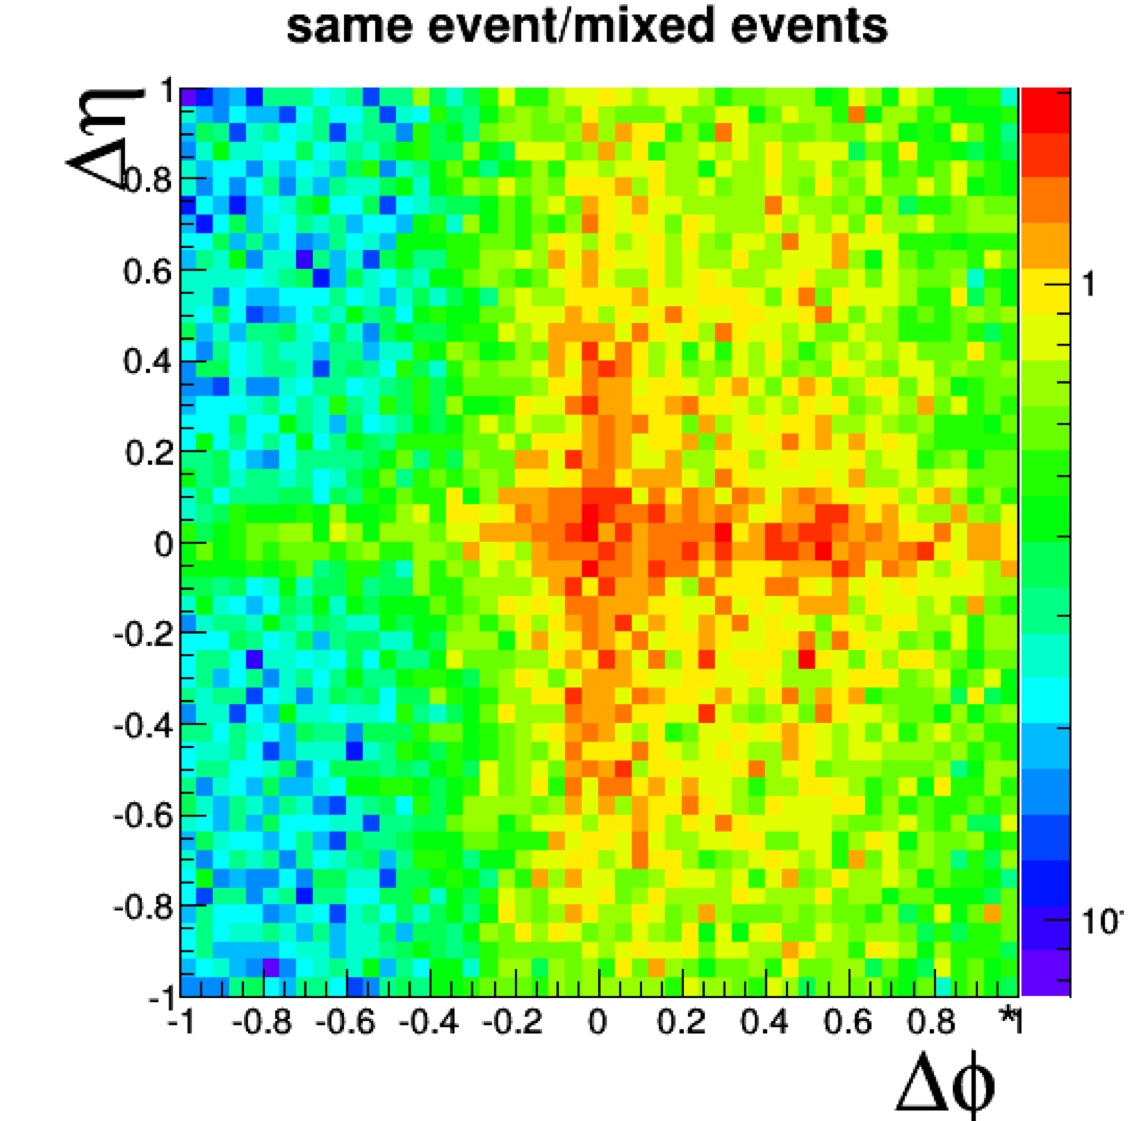
\includegraphics[width=.75\linewidth]{test_DEltaEta_DEltaphi.png}
      \end{figure}
    \end{block}
    \column{.48\textwidth}
    \begin{block}{\bf \centering How it should look:}
      \begin{figure}[H]
        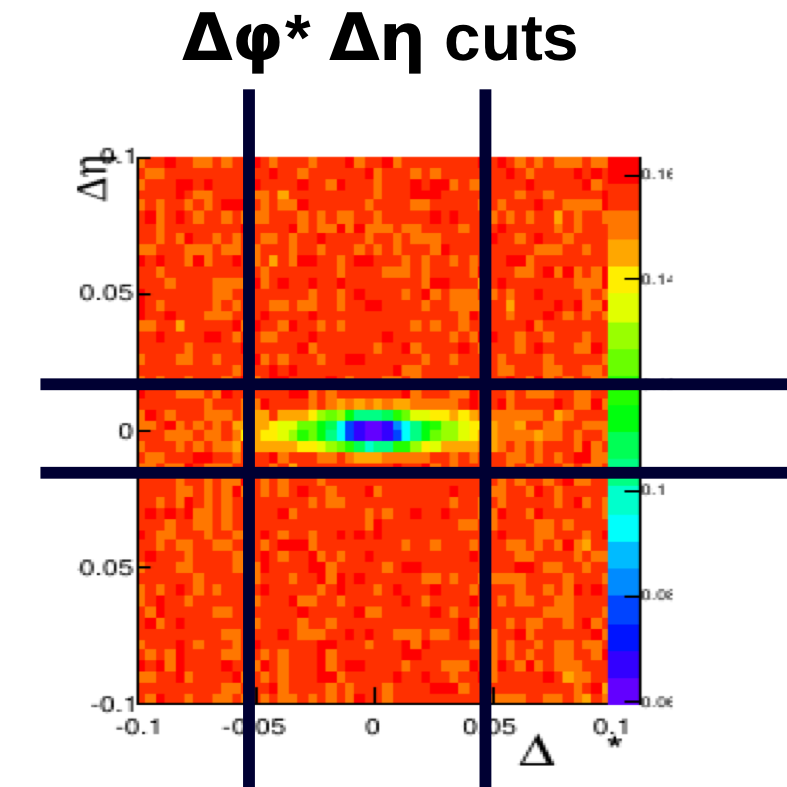
\includegraphics[width=.75\linewidth]{deltaEtadeltaPhi_howto.png}
      \end{figure}
    \end{block}
  \end{columns}
  \begin{block}{}
    \bf \centering
    {\LARGE
    The merging is not visible due to a very strong splitting.
    
    Firstly, we need to suppress the splitting!

    }
  \end{block}
\end{frame}
\end{document} 
